% this file is called up by thesis.tex
% content in this file will be fed into the main document

%: ----------------------- name of chapter  -------------------------
\chapter{Implementacja projektów} % top level followed by section, subsection


%: ----------------------- paths to graphics ------------------------

% change according to folder and file names
\ifpdf
    \graphicspath{{5/figures/PNG/}{5/figures/PDF/}{5/figures/}}
\else
    \graphicspath{{5/figures/EPS/}{5/figures/}}
\fi

%: ----------------------- contents from here ------------------------


W rozdziale trzecim zostały przedstawione wymagania funkcjonalne i niefunkcjonalne stawiane przed przykładowymi aplikacjami mogącymi korzystać z systemu którego implementacja była celem tej pracy. Niniejszy rozdział opisuje sposób implementacji tych aplikacji.
\section{Automatyczne dyktando}
Automatyczne dyktando, jak już zostało opisane w rozdziale trzecim, jest to prosty serwis internetowy umożliwiający użytkownikowi ćwiczenie ortografii. Jak większość współczesnych aplikacji internetowych ma budowę warstwową, składa się z 3 warstw:
\begin{itemize}
	\item prezentacji,
	\item logiki biznesowej,
	\item komunikacji z serwisem UniversalSynthesizer.
\end{itemize}
\begin{figure}[!h]
	\centering
	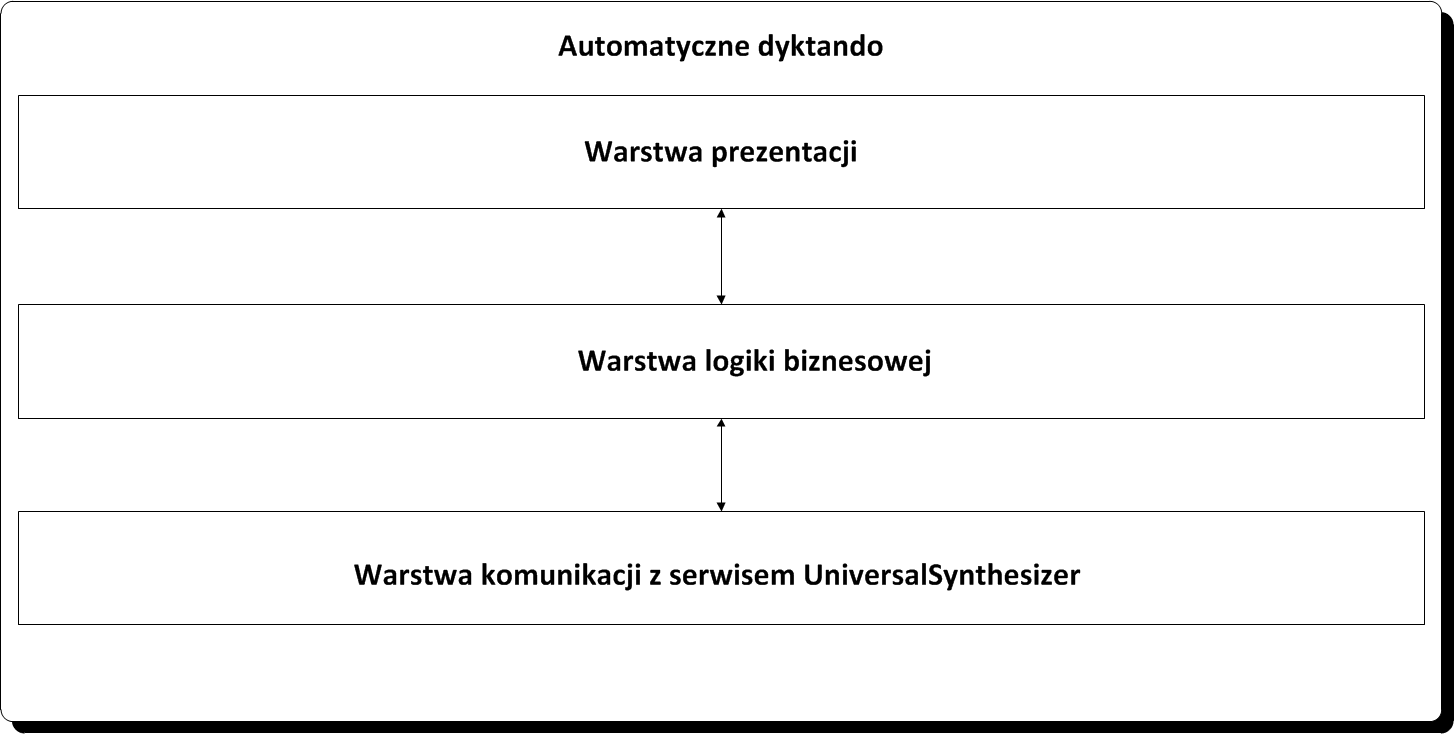
\includegraphics[scale=0.45]{automatyczneDyktandoArchitektura.png} 
	\caption{Automatyczne Dyktanto Architektura}
\end{figure}
Do stworzenia szkieletu tej aplikacji wykorzystano framework Spring MVC, do tworzenia widoków framework Freemarker a do komunikacji z serwisem UniversalSyntesizer bibliotekę jersey-client będącą implementacją JAX-RS. 
\newpage
\subsection{Warstwa prezentacji}
W skład warstwy prezentacji wchodzą trzy strony:
\begin{itemize}
	\item strona główna - umożliwiająca podanie tekstu lub też załadowanie pliku tekstowego, który posłuży jako treść dyktanda
	\item strona z odtwarzaczem - umożliwiająca odsłuchanie tekstu i napisanie jego transkrypcji
	\item strona z wynikami - pokazująca ilość błedów popełnionych przez użytkownika
\end{itemize}
Dodatkowo z każdej z wyżej wymienionych stron istnieje możliwość powrotu do głównej. \\
Jak już wspomniano wyżej, do przygotowania widoków użyto szablonów Freemarker'owych, po jednym na każdą z wymienionych stron, plus jeden dodatkowy, przeznaczonydo ładowania plików na serwer. Dzięki wykorzystaniu Spring MVC i wsparciu które zapewnia implementacja kontrolerów i możliwego przepływu sterowania była sprawą trywialną. s
\subsection{Warstwa logiki biznesowej}

\subsection{Warstwa komunikacji z serwisem UniversalSynthesizer}

\section{LektorsRSS}

\section{LektorSMS}




% ---------------------------------------------------------------------------
%: ----------------------- end of thesis sub-document ------------------------
% ---------------------------------------------------------------------------

